\documentclass[twoside, titlepage]{article}

\usepackage[margin=0.5in]{geometry}
\usepackage{fancyhdr}
\usepackage{lipsum}
\usepackage{graphicx}
\usepackage{caption}
\usepackage{setspace}
\usepackage{lastpage}
\usepackage{booktabs}
\usepackage{color}
\usepackage{colortbl}

\newcommand{\OOS}{Mumble Client}
\newcommand{\usabilitymethod}{[Usability Method]}
\newcommand{\mytitle}{An Assesment of the Design Quality and Usability of \OOS}
\newcommand{\myname}{Timothy Heath}

\pagestyle{fancy}
\fancyfoot[LE]{Heath}
\fancyfoot[R]{Page \thepage \ of \pageref{LastPage}}
\fancyfoot[C]{}
\fancyfoot[LO]{\mytitle}

\definecolor{yellow-green}{rgb}{0.35,0.35,0.35}
\definecolor{gray}{rgb}{0.75,0.75,0.75}

\title{\mytitle}
\author{\myname}
\date{\today}

\onehalfspacing
\begin{document}
%	\begin{titlepage}
%		{\centering\Huge\textbf{\mytitle}\par}
%		\vspace{1em}
%		\textbf{\myname}\par
%		\vspace{1em}
%		\lipsum[1-3] % TODO Replace with abstract
%	\end{titlepage}
%	\lipsum[4-9]
	\section*{The Design of \OOS}
	This section of the document will have
	two columns. The first holding the text,
	the second holding images for the reader.
	First this will explain what the Object
	of Study for this document is. Then this
	will cover some background information.
	Finally this will explain my own experience
	using this object.\newpage
	\begin{minipage}{0.5\textwidth}
		The Object of Study for this document is the
		default Mumble Client. This software runs on
		a computer in order to open a connection to
		a Murmur Server. This software serves to let
		multiple people talk to each other over computer
		networks, basically it is a light weight discord.\\
		
		
		This software is used to organize general chatrooms,
		enable teams to talk to each other while playing
		games, or just as an overkill VOIP phone. I have
		a murmur server running on my home network from
		my computer for playing video games with my family
		(I could open it to the internet, but I do not need
		to), you see a ping of zero in Figure \ref{fig:mumbleOpen} because the client used to view
		the connections is already on the computer running the
		server so there is no time lost in the network.\\
		
		
		Figure \ref{fig:mumbleOpen} shows the window that opens
		when the Mumble Client is started. I have used this
		software on multiple operating systems, the only
		difference on all of them has been the
		window decorations assigned to the window on
		creation, this is managed however by the window
		manager and has nothing to do with the actual
		software. The software in my experience is exactly
		the same on MS Windows and every distribution
		of Linux that I have run it on.\\
		
		The Mumble Client allows you to disconnect and connect
		to Murmur Servers, rather than only connecting to a
		singular server and disconnecting on close. Each time
		a connection is made from a client to a server, the
		user is prompted for a user-name. This user-name will
		serve to identify the messages from the user, and
		when the user is speaking, an indicator based on the
		user-name will toggle to show that there is audio
		coming from that user. Figure \ref{fig:mumbleConnected}
		shows the window after connecting to the server.\\
		
		A nice little feature shown in Figure
		\ref{fig:mumbleRecording} is that the Mumble client
		can record audio and save the file locally. One thing
		to mention about the Murmur Server and Mumble Clients
		is that they allow the use of multiple chat rooms under
		the Root in a tree structure.
	\end{minipage}
	\begin{minipage}{0.5\textwidth}
		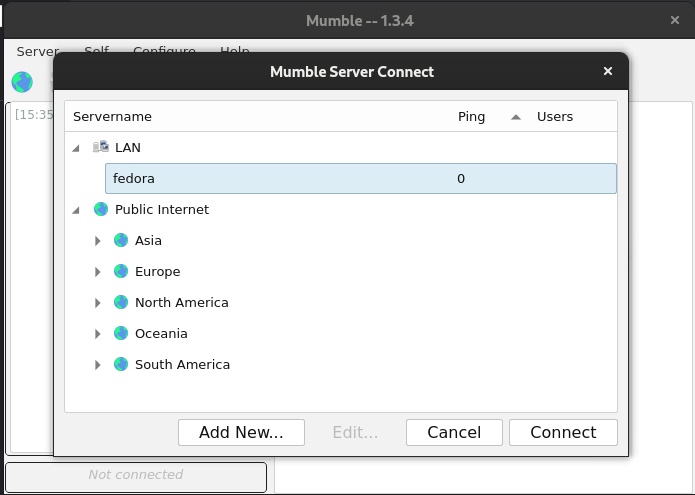
\includegraphics[width=4in]{resources/mumbleOpen}
		\captionof{figure}{This is the window that opens by
			default when you start the Mumble Client.}
		\label{fig:mumbleOpen}
		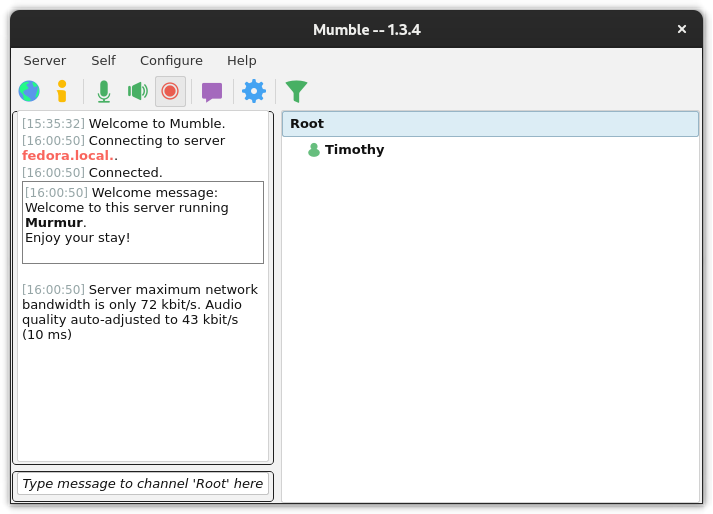
\includegraphics[width=4in]{resources/mumbleConnected}
		\captionof{figure}{This is the window shown after a
		connection to a Murmur Server is established.}
		\label{fig:mumbleConnected}
		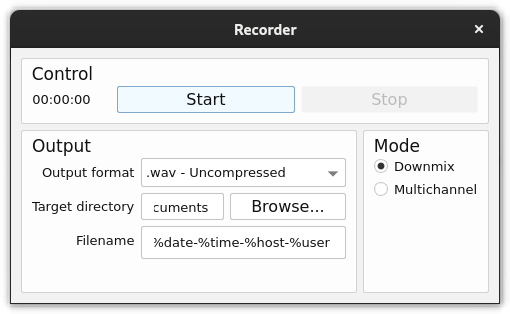
\includegraphics[width=4in]{resources/mumbleRecord}
		\captionof{figure}{This is the recording sub-window.}
		\label{fig:mumbleRecording}
	\end{minipage}
	\newpage
	\begin{tabular}[t]{ll}\toprule
		\rowcolor{yellow-green}
		Key Features & Description \\
		\rowcolor{gray}
		Per-Channel Instant Messaging & \begin{minipage}{0.5\textwidth}
			Each user on the server, being in a given
			chat-room may send and receive text messages
			to and from all users in the same chat room.
		\end{minipage}. \\\\
		Per-Channel Voice Chat & \begin{minipage}{0.5\textwidth}
			Each user on the server, being in a given
			chat-room may broadcast his voice to the entire
			chat-room.
		\end{minipage}. \\\\
		\rowcolor{gray}
		Channel Audio Recording & \begin{minipage}{0.5\textwidth}
			Each user on the server, being in a given
			chat-room may record all audio being played
			in the chat-room.
		\end{minipage}. \\\\
		User Registration & \begin{minipage}{0.5\textwidth}
			Each user may optionally register himself
			unto the server with a permanent user-name.
		\end{minipage}. \\\\
		\rowcolor{gray}
		User Comment & \begin{minipage}{0.5\textwidth}
			Each user may optionally create a comment
			that will be displayed next to his name in the 
			chat-room.
		\end{minipage}. \\\\
		User Avatar & \begin{minipage}{0.5\textwidth}
			Each user on the server, being in a given
			chat-room may set an avatar for himself to be
			displayed when anyone hovers his mouse over his
			icon.
		\end{minipage}. \\\\
		\rowcolor{gray}
		Interface Customization & \begin{minipage}{0.7\textwidth}
			The desktop Mumble interface is fully customizable.
		\end{minipage}. \\\\
		Positional Audio & \begin{minipage}{0.5\textwidth}
			When running the Mumble Client in a supported
			game, audio from people playing the same game will
			sound as if it came from their in-game location.
		\end{minipage}. \\\\
		\rowcolor{gray}
		Opus Codec & \begin{minipage}{0.5\textwidth}
			Use of the free Opus Codec by default prioritizes
			low-latency and high-quality audio transmission.
		\end{minipage}. \\\\
		Noise Suppression & \begin{minipage}{0.5\textwidth}
			When connected to a chat-room, noise below a
			chosen threshold will not be broadcast.
		\end{minipage}. \\\\
		\rowcolor{gray}
		Automatic Level Balancing & \begin{minipage}{0.5\textwidth}
			At the server, attempts are made to set all volumes
			from each user to an equal level in order to
			prevent one user drowning out all others when
			talking.
		\end{minipage}. \\\\
		Attenuation & \begin{minipage}{0.5\textwidth}
			Optionally a user of the client may have it lower
			volume from other applications while receiving
			audio from other users.
		\end{minipage}. \\\\
		\rowcolor{gray}
		Priority Speakers & \begin{minipage}{0.5\textwidth}
			On the server, certain users may be given a
			priority status enabling their voice to win out
			over others when conflict occurs.
		\end{minipage}. \\\\
		Encryption & \begin{minipage}{0.5\textwidth}
			All data transmitted to and from the server
			is encrypted, this ensures that the privacy of the
			group is legally protected from those disconnected
			from the server.
		\end{minipage}. \\\\
		\rowcolor{gray}
		Setup Wizards & \begin{minipage}{0.5\textwidth}
			At set up of the client for the first time, a
			sequence of wizards configure the client to
			the user's liking.
		\end{minipage}. \\\\
		Authentication & \begin{minipage}{0.5\textwidth}
			By using certificates for authenticating, two
			friends may see each other by friends on a server,
			even if they go by different names on that other 
			server.
		\end{minipage}. \\\\
		\rowcolor{gray}
		Server List & \begin{minipage}{0.5\textwidth}
			Mumble has a public server list sorted by nation
			that users may add private servers to for easy 
			access.
		\end{minipage}. \\\\
	\end{tabular}
	\newpage
	\begin{tabular}[t]{ll}\toprule
		\rowcolor{yellow-green}
		Key Functions & Description \\
		\rowcolor{gray}
		Instant Messaging & \begin{minipage}{0.5\textwidth}
			Each user may broadcast instant messages to the
			current channel he is in.
		\end{minipage}. \\\\
		Voice Chat & \begin{minipage}{0.5\textwidth}
			Each user may broadcast his voice to the current
			channel.
		\end{minipage}. \\\\
		\rowcolor{gray}
		Audio Recording & \begin{minipage}{0.5\textwidth}
			The client may record the audio from the connected
			channel.
		\end{minipage}. \\\\
		User Registration & \begin{minipage}{0.5\textwidth}
			Register the user permanently to the server with
			a permanent name.
		\end{minipage}. \\\\
		\rowcolor{gray}
		User Profile & \begin{minipage}{0.5\textwidth}
			Each user may optionally create a comment
			that will be displayed next to his name in the 
			chat-room.
		\end{minipage}. \\\\
		User Avatar & \begin{minipage}{0.5\textwidth}
			Each user on the server, being in a given
			chat-room may set an avatar for himself to be
			displayed when anyone hovers his mouse over his
			icon.
		\end{minipage}. \\\\
		\rowcolor{gray}
		Interface Customization & \begin{minipage}{0.5\textwidth}
			The desktop Mumble interface is fully customizable.
		\end{minipage}. \\\\
		Positional Audio & \begin{minipage}{0.5\textwidth}
			When running the Mumble Client in a supported
			game, audio from people playing the same game will
			sound as if it came from their in-game location.
		\end{minipage}. \\\\
		\rowcolor{gray}
		Low-Latency, High-Quality Audio Transmission & \begin{minipage}{0.5\textwidth}
			Use of the free Opus Codec by default prioritizes
			low-latency and high-quality audio transmission.
		\end{minipage}. \\\\
		Noise Suppression & \begin{minipage}{0.5\textwidth}
			When connected to a chat-room, noise below a
			chosen threshold will not be broadcast.
		\end{minipage}. \\\\
		\rowcolor{gray}
		Automatic Level Balancing & \begin{minipage}{0.5\textwidth}
			At the server, attempts are made to set all volumes
			from each user to an equal level in order to
			prevent one user drowning out all others when
			talking.
		\end{minipage}. \\\\
		Attenuation & \begin{minipage}{0.5\textwidth}
			Optionally a user of the client may have it lower
			volume from other applications while receiving
			audio from other users.
		\end{minipage}. \\\\
		\rowcolor{gray}
		Priority Speakers & \begin{minipage}{0.5\textwidth}
			On the server, certain users may be given a
			priority status enabling their voice to win out
			over others when conflict occurs.
		\end{minipage}. \\\\
		Encryption & \begin{minipage}{0.5\textwidth}
			All data transmitted to and from the server
			is encrypted, this ensures that the privacy of the
			group is legally protected from those disconnected
			from the server.
		\end{minipage}. \\\\
		\rowcolor{gray}
		Setup Wizards & \begin{minipage}{0.5\textwidth}
			At set up of the client for the first time, a
			sequence of wizards configure the client to
			the user's liking.
		\end{minipage}. \\\\
		Security & \begin{minipage}{0.5\textwidth}
			Communication via the server is legally secure
			in that communication is private and the source
			is verifiable.
		\end{minipage}. \\\\
		\rowcolor{gray}
		Server List & \begin{minipage}{0.5\textwidth}
			Mumble has a public server list sorted by nation
			that users may add private servers to for easy 
			access.
		\end{minipage}. \\\\
	\end{tabular}
%	\section*{Heuristic Analyses of \OOS}
%	\section*{\usabilitymethod\ Analyses of the \OOS}
%	\section*{Lessons Learned About the Design and Usability of \OOS}
\end{document}
